% =============================================================================
%  CHAPITRE 3 : PRÉSENTATION DU SITE DE L'ÉTUDE, DES DONNÉES ET DES RÉSULTATS
%
%  Structure imposée par le « Guide de rédaction KEYCE v3.0 » (§ 13 et § 14) :
%      Introduction
%      3.1. Présentation du site de l'étude
%      3.2. Présentation des données et des résultats
%      Conclusion
% =============================================================================
\entete{Chapitre 3 : Site de l'étude, données et résultats}
\chapter{Présentation du site de l'étude, des données et des résultats}
\label{chap:terrain}

\introchap

Ce chapitre confronte au terrain la démarche exposée précédemment. Il présente
d'abord le site de l'étude, c'est-à-dire la Fondation Jean Félicien Gacha et
son Département \emph{Think Tank} Fou'ndjem, qui nous a accueilli. Il expose
ensuite les données recueillies auprès du personnel et des visiteurs,
l'implémentation du dispositif construit à partir de ces données, puis les
résultats obtenus. La présentation reste ici factuelle : son interprétation au
regard des hypothèses de l'étude est réservée au chapitre~\ref{chap:diagnostic}.

% =============================================================================
\section{Présentation du site de l'étude}
\label{sec:site}

\subsection{Identification de la structure}

La Fondation Jean Félicien Gacha est une organisation à but non lucratif de
droit camerounais implantée à Bangoulap, dans l'arrondissement de Bangangté,
département du Ndé, région de l'Ouest du Cameroun. Elle intervient dans la
culture, l'art, l'artisanat, l'éducation et le développement communautaire. Le
tableau~\ref{tab:fiche} en présente la fiche d'identification.

\begin{table}[htbp]
\centering
\caption{Fiche d'identification de la Fondation Jean Félicien Gacha}
\label{tab:fiche}
\small
\begin{tabularx}{\textwidth}{|L{5.2cm}|X|}
\hline
\rowcolor{keycetete}
\thead{Désignation} & \thead{Affectation} \\ \hline
Dénomination & Fondation Jean Félicien Gacha \\ \hline
Nature juridique & Fondation, organisation à but non lucratif \\ \hline
Secteur d'activité & Culture, art, artisanat, éducation, développement communautaire \\ \hline
Siège & Bangoulap, arrondissement de Bangangté, département du Ndé, région de l'Ouest \\ \hline
Pays & Cameroun \\ \hline
% À COMPLÉTER AVANT REMISE (exigé par le guide, § 13) : décommenter et renseigner.
% Date de création & \dots \\ \hline
% Effectif du personnel & \dots \\ \hline
Domaines d'intervention & Espaces d'exposition, ateliers de création, résidences d'artistes, espaces verts, actions communautaires \\ \hline
Entité d'accueil du stage & Département \emph{Think Tank} Fou'ndjem \\ \hline
Encadreur professionnel & M. Adrien GHOMSI \\ \hline
Période du stage & Du 20 juin au 20 août 2026 \\ \hline
\end{tabularx}
\source{Documents internes de la Fondation et entretiens, juin 2026.}
\end{table}

Deux éléments de cette fiche commandent la suite du travail : la Fondation
détient un patrimoine exposé sur un site unique, dont la découverte suppose un
déplacement ; et l'entité qui nous a accueilli n'est pas un service
d'exploitation, mais un département de réflexion.

\subsection{Historique, missions et organisation}

La Fondation porte le nom de son initiateur, Jean Félicien Gacha, dont l'action
visait à faire de Bangoulap un lieu de rencontre entre la création
contemporaine et les savoir-faire hérités des chefferies de l'Ouest. Née d'une
initiative privée, la structure s'est progressivement dotée d'espaces
d'exposition, d'ateliers et de résidences, puis a élargi son action au
développement communautaire : sa trajectoire va de la collection privée à
l'institution ouverte au public, puis à l'acteur du développement territorial.
Elle explique le trait saillant du terrain sur lequel s'appuie toute notre
intervention : un patrimoine matériel et documentaire considérable, mais une
organisation encore fondée sur la mémoire des personnes et sur des supports non
structurés.

Ses missions se regroupent en quatre ensembles : \textbf{conserver et présenter}
le patrimoine de l'Ouest camerounais ; \textbf{soutenir la création}, par
l'accueil d'artistes en résidence ; \textbf{transmettre}, envers les scolaires,
les chercheurs et les visiteurs ; et contribuer au \textbf{développement
communautaire} local.

Sur le plan organisationnel, la Fondation s'articule autour d'une direction, de
pôles opérationnels — conservation et exposition, ateliers et résidences,
accueil du public, communication, administration et finances — et d'un
département de réflexion rattaché à la direction, le \emph{Think Tank}
Fou'ndjem (figure~\ref{fig:organigramme}).

\begin{figure}[htbp]
\centering
\schema{organigramme}
\caption{Organigramme de la Fondation Jean Félicien Gacha}
\label{fig:organigramme}
\source{Élaboré par nos soins à partir des entretiens conduits en juin 2026.}
\end{figure}

\subsection{Le Département \emph{Think Tank} Fou'ndjem et son rôle dans le projet}
\label{sec:thinktank}

Le Département \emph{Think Tank} Fou'ndjem est la structure de la Fondation
dédiée à la réflexion et à la recherche sur les questions relatives au
Cameroun, à sa culture, à son patrimoine et à son développement. Il constitue
un espace de veille et d'analyse où sont examinées les problématiques
contemporaines susceptibles d'éclairer les grands enjeux du pays, notamment
celles qui touchent à la modernisation des infrastructures et au développement
technologique et économique.

C'est dans ce cadre que le Département nous a accueilli pour notre stage
académique. Son rôle dans le projet n'a pas été celui d'un client
opérationnel : il n'administre pas les collections, ne reçoit pas le public et
n'est pas l'utilisateur final de la plateforme, fonctions qui relèvent des
pôles Conservation et exposition, Accueil du public et Communication. Il a
tenu, lui, le rôle d'un cadre d'encadrement intellectuel et méthodologique.
C'est notre encadreur au sein de ce Département, M. Adrien GHOMSI, qui nous a
proposé de faire mûrir et d'approfondir un thème initialement esquissé, pour en
faire un véritable sujet de fin d'études aligné sur notre spécialité en génie
informatique.

Notre travail a dès lors consisté à contextualiser cette réflexion : concevoir
et développer une plateforme de valorisation numérique du patrimoine adaptée
aux réalités camerounaises — connectivité mobile instable, coût des données,
sécurité des données en environnement multi-institutions — et montrer
concrètement comment les enjeux de développement technologique portés par le
\emph{Think Tank} Fou'ndjem peuvent se traduire en solutions logicielles
souveraines et contextualisées. Ces trois contraintes ne sont pas restées
théoriques : elles ont commandé la priorité donnée au téléphone mobile, la
sobriété des médias transportés et le cloisonnement des données par
institution, décrits à la section~\ref{sec:implementation}.

Le Département a donc joué un rôle de structure d'accueil et d'orientation
scientifique : il a validé la pertinence du sujet et nous a laissé la liberté
méthodologique nécessaire pour le développer techniquement, sans intervenir
dans les choix d'implémentation, qui relèvent strictement de notre spécialité.
Le tableau~\ref{tab:entites} situe les entités de la Fondation concernées par
l'étude.

\begin{table}[htbp]
\centering
\caption{Entités de la Fondation concernées par l'étude}
\label{tab:entites}
\small
\begin{tabularx}{\textwidth}{|L{3.6cm}|L{4.4cm}|X|}
\hline
\rowcolor{keycetete}
\thead{Entité} & \thead{Rôle dans l'organisation} & \thead{Lien avec l'étude} \\ \hline
Direction & Conduite de la Fondation & Ouverture des espaces et des archives ; validation du principe du projet \\ \hline
Département \emph{Think Tank} Fou'ndjem & Réflexion, veille et recherche sur le patrimoine et le développement & Structure d'accueil du stage ; cadrage intellectuel et méthodologique du sujet \\ \hline
Pôle Conservation et exposition & Collections, salles et notices & Source de la matière documentaire ; utilisateur final du back-office \\ \hline
Pôle Accueil du public & Visites guidées, entrées, ventes d'artisanat & Terrain d'observation ; utilisateur final de la billetterie et de la boutique \\ \hline
Pôle Communication & Présence en ligne de la Fondation & Utilisateur final du site public et des campagnes d'information \\ \hline
\end{tabularx}
\source{Élaboré par nos soins à partir des entretiens conduits en juin 2026.}
\end{table}

Le tableau~\ref{tab:entites} distingue le cadre d'accueil du périmètre
d'application : le Département a cadré et validé la question de recherche,
tandis que les pôles opérationnels ont fourni la matière documentaire et
constituent les utilisateurs finaux du dispositif. Cette distinction écarte un
contresens fréquent, qui consisterait à prendre l'entité d'accueil pour le
commanditaire fonctionnel.

\subsection{Environnement technologique existant}

Le relevé de l'environnement numérique de la Fondation, effectué durant la
première semaine du stage, fait apparaître la situation suivante :

\begin{itemize}
  \item \textbf{aucun système de gestion des collections} : l'inventaire des
        œuvres est tenu sur des supports bureautiques dispersés et sur des
        cahiers ;
  \item \textbf{une présence en ligne réduite} : quelques pages de présentation
        et des publications sur les réseaux sociaux, sans base documentaire ;
  \item \textbf{aucune billetterie ni boutique en ligne} : les entrées et les
        ventes d'artisanat se traitent exclusivement sur place ;
  \item \textbf{aucun fichier des visiteurs} : une personne ayant visité la
        Fondation ne peut pas être recontactée pour être informée d'une
        exposition ;
  \item \textbf{aucune sauvegarde structurée} des photographies et des notices.
\end{itemize}

Le contexte de collecte est donc celui d'une institution \emph{sans} système
d'information : les données de l'étude ont été recueillies auprès des personnes
et sur des supports non structurés, et non extraites d'une base existante. Ce
point commande à la fois la méthode suivie et l'ampleur du travail de saisie
initial.

\subsection{Cadre et déroulement du stage}
\label{sec:stage}

Le stage s'est déroulé du 20 juin au 20 août 2026. Il a débuté par un entretien
avec M. Adrien GHOMSI, consacré aux attentes de la structure, au règlement
intérieur et aux objectifs de la période. Une visite complète des espaces,
conduite par le pôle Accueil du public, nous a permis de prendre la mesure du
lieu — condition préalable à toute tentative de le restituer numériquement — et
d'observer dès la première semaine des visites guidées réelles ainsi que les
questions que les visiteurs y posent spontanément. Les travaux ont ensuite été
supervisés par l'encadreur professionnel selon le programme hebdomadaire
présenté au tableau~\ref{tab:chronogramme}.

\begin{table}[htbp]
\centering
\caption{Chronogramme des tâches effectuées durant le stage}
\label{tab:chronogramme}
\footnotesize
\begin{tabularx}{\textwidth}{|L{3.4cm}|X|}
\hline
\rowcolor{keycetete}
\thead{Période} & \thead{Tâches effectuées} \\ \hline
Du 20 au 26 juin 2026 &
Accueil et présentation de la Fondation ; prise de contact avec le personnel du
Département \emph{Think Tank} Fou'ndjem ; visite complète des espaces ; cadrage
du sujet avec l'encadreur professionnel ; observation de visites guidées. \\ \hline
Du 27 juin au 3 juillet 2026 &
Étude de l'existant ; entretiens semi-directifs avec six membres du personnel ;
relevé de l'environnement numérique ; dépouillement des inventaires et des
notices ; administration du questionnaire aux visiteurs. \\ \hline
Du 4 au 10 juillet 2026 &
Rédaction du cahier des charges ; arbitrage des besoins avec l'encadreur
professionnel ; choix de l'architecture et des technologies. \\ \hline
Du 11 au 17 juillet 2026 &
Conception et création de la base de données ; mise en place du cloisonnement
par organisation ; développement du back-office : musées, salles, œuvres,
tarifs, médias. \\ \hline
Du 18 au 24 juillet 2026 &
Développement du site public ; catalogue, fiches d'œuvres, boutique,
billetterie avec billets à code QR ; gestion des événements et du livre d'or. \\ \hline
Du 25 au 31 juillet 2026 &
Développement du moteur de visite immersive à 360~degrés ; éditeur de parcours
dans le back-office ; pose des points d'intérêt ; enchaînement des salles. \\ \hline
Du 1\textsuperscript{er} au 7 août 2026 &
Numérisation en trois dimensions ; réalité augmentée ; génération des codes QR ;
essais de photogrammétrie et d'acquisition par capteur LiDAR ; couverture des
appareils Android et iOS. \\ \hline
Du 8 au 14 août 2026 &
Développement de l'assistant conversationnel à ancrage documentaire ;
rapprochement documentaire avec les collections ouvertes ; module de généalogie ;
campagnes d'information aux adhérents. \\ \hline
Du 15 au 20 août 2026 &
Conteneurisation ; chaînes d'intégration et de déploiement continus ;
description de l'infrastructure ; mise en ligne ; essais de bout en bout ;
mesures de performance et de coût ; restitution à l'encadreur professionnel. \\ \hline
\end{tabularx}
\source{Journal de bord du stage, juin--août 2026.}
\end{table}

Le chronogramme fait apparaître l'économie de la période : trois semaines
consacrées au terrain et au cadrage, six semaines de réalisation menées par
ordre de priorité décroissante des attentes recueillies, et une dernière
semaine d'industrialisation, de mise en ligne et de mesure.

\paragraph{Justification du choix du terrain.} Trois caractéristiques font de
ce terrain un cas instructif. La richesse patrimoniale y est réelle et
documentée, ce qui écarte le risque de construire un dispositif sans matière.
Les contraintes de moyens y sont représentatives de celles des institutions
patrimoniales de la sous-région, de sorte que ce qui fonctionne ici a des
chances de fonctionner ailleurs. Enfin, le Département \emph{Think Tank}
Fou'ndjem garantissait un interlocuteur capable de formuler le besoin et
d'arbitrer les choix, condition indispensable à une recherche interactive.

% =============================================================================
\section{Présentation des données et des résultats}
\label{sec:donnees}

\subsection{Les données recueillies}

\subsubsection{Étude de l'existant}

L'étude de l'existant consiste à analyser les outils, les processus et les
systèmes en place afin d'en identifier les forces, les faiblesses et les besoins
non satisfaits. Appliquée à la Fondation, elle révèle un fonctionnement
entièrement manuel pour ce qui touche à la valorisation.

La découverte des espaces suppose une visite sur place. Les collections ne sont
inventoriées que partiellement, sur des supports non reliés entre eux. Les
tarifs et les entrées sont gérés sur registre papier. La communication vers le
public repose sur des publications ponctuelles sur les réseaux sociaux, sans
possibilité de recontacter les personnes intéressées. Enfin, aucune information
n'est disponible pour le visiteur en dehors de la présence d'un guide.

Le tableau~\ref{tab:existant} récapitule les insuffisances relevées et les
besoins qui en découlent.

\begin{table}[htbp]
\centering
\caption{Insuffisances du dispositif existant et besoins induits}
\label{tab:existant}
\small
\begin{tabularx}{\textwidth}{|L{4.4cm}|X|L{3.4cm}|}
\hline
\rowcolor{keycetete}
\thead{Domaine} & \thead{Insuffisance constatée} & \thead{Besoin induit} \\ \hline
Accès au lieu & La visite exige un déplacement physique & Parcours immersif à distance \\ \hline
Perception des œuvres & Photographies plates, aucune notion de volume ni de taille & Présentation en trois dimensions et en réalité augmentée \\ \hline
Documentation & Notices dispersées, objets traités isolément & Inventaire structuré et mise en relation \\ \hline
Information du visiteur & Aucune réponse possible hors présence d'un guide & Assistant conversationnel ancré sur les documents \\ \hline
Gestion administrative & Registres papier, données non sauvegardées & Progiciel de gestion intégré \\ \hline
Relation au public & Aucun fichier de visiteurs & Adhésion en ligne et campagnes d'information \\ \hline
Rayonnement & Dispositif non transposable à d'autres institutions & Architecture ouverte à plusieurs organisations \\ \hline
\end{tabularx}
\source{Étude de l'existant, juin--juillet 2026.}
\end{table}

Le tableau~\ref{tab:existant} met en évidence un enchaînement : chaque
insuffisance relevée appelle un besoin précis, et chacun de ces besoins se
retrouve plus loin sous la forme d'une fonctionnalité livrée. Les sept lignes
couvrent l'accès au lieu, la perception des œuvres, la documentation,
l'information du visiteur, la gestion administrative, la relation au public et
le rayonnement de l'institution : le déficit n'est donc pas ponctuel, il est
systémique.

\subsubsection{Résultats des entretiens}

L'analyse thématique des six entretiens conduits auprès du personnel a fait
émerger cinq thèmes, présentés ici par ordre de fréquence d'apparition.

\begin{enumerate}
  \item \textbf{L'accessibilité} (six entretiens sur six). Le déplacement est
        unanimement désigné comme le premier obstacle ; la diaspora, les
        chercheurs étrangers et les écoles éloignées sont explicitement cités.

  \item \textbf{La perception de l'espace} (cinq entretiens). Une photographie
        ne rend compte ni des volumes ni de l'atmosphère des salles ;
        l'expression « il faut être là pour comprendre » revient plusieurs fois.

  \item \textbf{La mise en relation des objets} (quatre entretiens). Ce thème
        n'était pas anticipé : il est apparu lorsqu'un interlocuteur a évoqué
        des pièces comparables conservées à l'étranger, dont la Fondation n'a
        connaissance que par ouï-dire. Cette remarque a engendré la deuxième
        question spécifique de l'étude.

  \item \textbf{La fiabilité de l'information} (quatre entretiens). Un
        dispositif automatique qui énoncerait des informations fausses
        porterait atteinte à la crédibilité de l'institution. Cette exigence a
        orienté toute la conception de l'assistant.

  \item \textbf{La pérennité économique} (trois entretiens) : le coût de
        fonctionnement une fois le stagiaire parti. Cette question justifie à
        elle seule la place accordée au FinOps dans ce travail.
\end{enumerate}

\subsubsection{Résultats du questionnaire}

Le questionnaire a été administré à 42 visiteurs. Le
tableau~\ref{tab:profil} présente le profil des répondants et le
tableau~\ref{tab:attentes} leurs attentes.

\begin{table}[htbp]
\centering
\caption{Profil des répondants au questionnaire}
\label{tab:profil}
\small
\begin{tabularx}{\textwidth}{|L{4.0cm}|X|C{2.2cm}|C{2.2cm}|}
\hline
\rowcolor{keycetete}
\thead{Caractéristique} & \thead{Modalité} & \thead{Effectif} & \thead{Fréquence} \\ \hline
\multirow{3}{*}{Tranche d'âge}
 & 18 à 30 ans & 19 & 45,2 \% \\ \cline{2-4}
& 31 à 45 ans & 15 & 35,7 \% \\ \cline{2-4}
& 46 ans et plus & 08 & 19,1 \% \\ \hline
\multirow{3}{*}{Provenance}
 & Région de l'Ouest & 21 & 50,0 \% \\ \cline{2-4}
& Autre région du Cameroun & 14 & 33,3 \% \\ \cline{2-4}
& Étranger & 07 & 16,7 \% \\ \hline
\multirow{2}{*}{Équipement principal}
 & Téléphone mobile & 36 & 85,7 \% \\ \cline{2-4}
& Ordinateur & 06 & 14,3 \% \\ \hline
\rowcolor{keycetotal}
\textbf{Total} & & \textbf{42} & \textbf{100 \%} \\ \hline
\end{tabularx}
\source{Enquête par questionnaire, juillet 2026.}
\end{table}

Deux enseignements ressortent de ce profil. D'une part, la moitié des visiteurs
vient déjà de l'extérieur de la région, ce qui atteste l'existence d'un public
prêt à s'intéresser à la Fondation à distance. D'autre part, plus de huit
visiteurs sur dix accèdent au numérique par un téléphone mobile : le dispositif
devait donc être conçu pour le téléphone en priorité, et non pour l'ordinateur.

\begin{table}[htbp]
\centering
\caption{Attentes exprimées à l'égard d'un dispositif de visite à distance}
\label{tab:attentes}
\small
\begin{tabularx}{\textwidth}{|X|C{2.4cm}|C{2.4cm}|}
\hline
\rowcolor{keycetete}
\thead{Attente exprimée} & \thead{Effectif} & \thead{Fréquence} \\ \hline
Se déplacer dans les salles comme si l'on y était & 38 & 90,5 \% \\ \hline
Voir les objets sous tous leurs angles et connaître leur taille réelle & 35 & 83,3 \% \\ \hline
Poser des questions et obtenir une réponse immédiate & 33 & 78,6 \% \\ \hline
Savoir à qui l'objet a appartenu et d'où il vient & 29 & 69,0 \% \\ \hline
Savoir si des objets semblables existent ailleurs dans le monde & 24 & 57,1 \% \\ \hline
Acheter un billet ou un objet d'artisanat en ligne & 18 & 42,9 \% \\ \hline
\end{tabularx}
\source{Enquête par questionnaire, juillet 2026, questions à réponses multiples.}
\end{table}

Ces résultats confirment la hiérarchie retenue dans les objectifs : la
restitution du déplacement dans l'espace arrive en tête, suivie de la perception
des objets, puis de la possibilité d'interroger. Ils valident également la
pertinence de la mise en relation entre institutions, souhaitée par plus d'un
visiteur sur deux alors même qu'elle ne figurait pas dans la demande initiale.

\subsection{L'implémentation du système}
\label{sec:implementation}

\subsubsection{Architecture générale de la plateforme}

L'architecture retenue comporte trois couches. Une \textbf{couche de
présentation} s'exécute dans le navigateur du visiteur : elle regroupe le site
public, le back-office et les moteurs de rendu écrits sur mesure. Une
\textbf{couche de services} regroupe la base de données, l'authentification et
douze fonctions serveur qui exécutent tout ce qui exige une clé d'accès ou un
privilège. Une \textbf{couche de diffusion} sert les fichiers statiques depuis
un réseau de distribution mondial.

Le principe directeur est simple et n'a jamais été enfreint : \emph{aucune clé
d'accès à un service tiers ne se trouve dans le navigateur}. Toute demande
adressée à un modèle de langue, à un service de synthèse vocale ou à un service
de paiement transite par une fonction serveur qui détient seule le secret.

\begin{figure}[htbp]
\centering
\schema{architecture-generale}
\caption{Architecture générale de la plateforme MUSÉA}
\label{fig:archi}
\source{Élaboré par nos soins.}
\end{figure}

\subsubsection{Architecture de l'assistant conversationnel à ancrage documentaire}

L'assistant repose sur une architecture de génération augmentée par la
recherche, dont le principe a été exposé au chapitre~1. Sa mise en œuvre suit
cinq temps.

\begin{enumerate}
  \item \textbf{Ingestion.} Les documents de référence de la Fondation (notices d'œuvres, descriptions de salles, histoires des musées,
        biographies des personnages, foire aux questions) sont exportés depuis
        la base de données et déposés dans un espace de stockage d'objets. Ce
        dépôt constitue la source de vérité documentaire : rien de ce qui n'y
        figure pas ne peut fonder une réponse.

  \item \textbf{Découpage et vectorisation.} Chaque document est découpé en
        fragments de taille homogène, puis converti en vecteur numérique par un
        modèle de plongement. Un point de méthode s'est révélé décisif : les
        fragments sont plongés \textbf{en anglais}. Les mesures conduites
        montrent en effet qu'une requête française classait une peinture sans
        rapport devant deux masques réellement apparentés, tandis qu'en anglais
        les correspondances légitimes atteignaient un score d'au moins 0,898
        contre au plus 0,779 pour le bruit, une étendue de 0,20 contre 0,13.

  \item \textbf{Indexation.} Les vecteurs sont enregistrés dans la base de
        données, dans une colonne vectorielle de dimension 384 dotée d'un index
        de type HNSW en distance cosinus. Cet index rend la recherche des plus
        proches voisins praticable sans parcourir l'ensemble des fragments.

  \item \textbf{Recherche et augmentation.} À la réception d'une question, la
        fonction serveur applique d'abord ses garde-fous : elle répond avec
        courtoisie aux salutations, refuse poliment les sujets hors périmètre,
        et restreint le cas échéant la recherche au musée ou à la salle où se
        trouve le visiteur. Elle convertit ensuite la question en vecteur,
        récupère les fragments les plus proches et compose l'instruction
        adressée au modèle de langue.

  \item \textbf{Génération contrôlée.} Le modèle rédige la réponse. La consigne
        lui interdit d'énoncer un fait absent des fragments fournis, lui impose
        de citer l'institution et le numéro d'inventaire lorsqu'ils existent, et
        l'autorise explicitement à déclarer qu'aucune conclusion n'est possible.
        Cette autorisation est essentielle : sans elle, un modèle de langue
        préfère inventer plutôt que de décevoir.
\end{enumerate}

\begin{figure}[htbp]
\centering
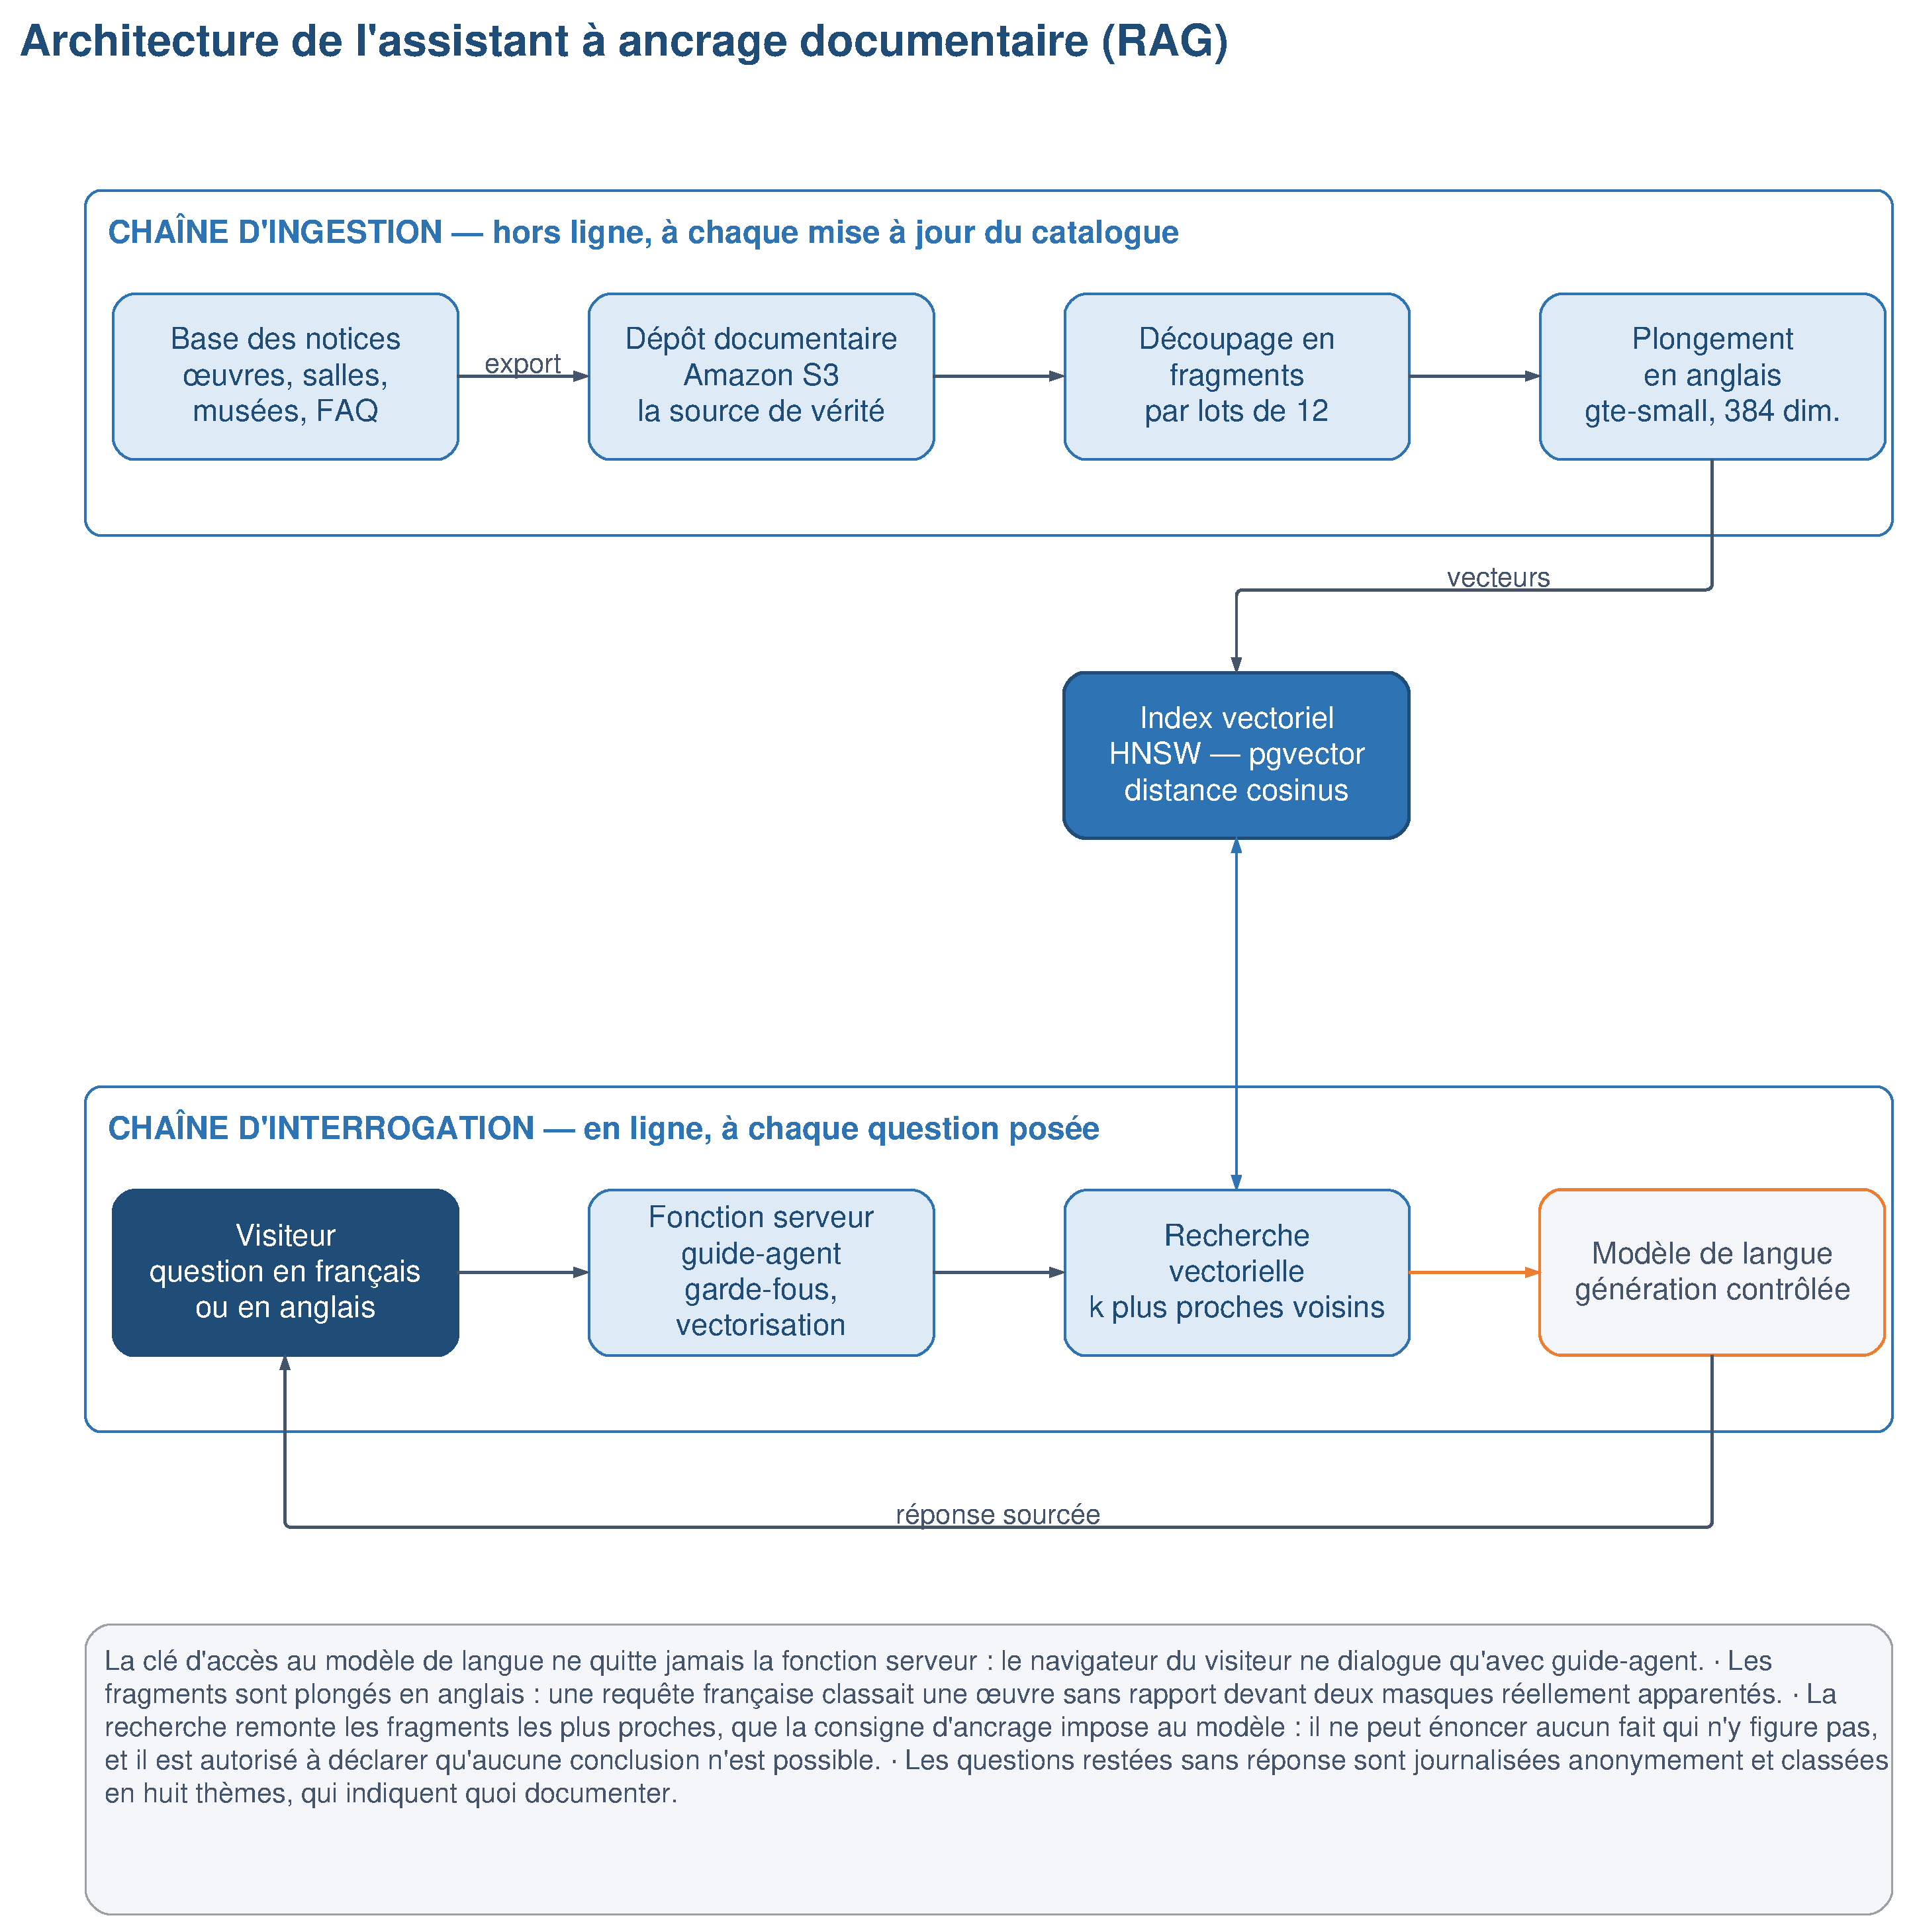
\includegraphics[width=\textwidth]{figures/rag-musea.pdf}
\caption{Architecture de l'assistant conversationnel à ancrage documentaire (RAG)}
\label{fig:rag}
\source{Élaboré par nos soins.}
\end{figure}

Une contrainte d'exploitation mérite d'être signalée, car elle a dicté un choix
d'implémentation. La plateforme d'exécution des fonctions serveur impose une
limite de ressources : la vectorisation de dix-huit fragments passe en
1,7~seconde, tandis que vingt fragments déclenchent l'interruption de la
fonction. Les traitements sont donc découpés en lots de douze, valeur retenue
avec une marge de sécurité délibérée.

\subsubsection{Le moteur de visite immersive}

L'impossibilité d'ajouter des bibliothèques a conduit à écrire le moteur de
panorama de bout en bout. Il restitue la salle sans aucun maillage, ce qui
supprime les défauts de facettes, et efface la couture verticale visible à la
jonction des bords de l'image. Les points d'intérêt ne sont pas dessinés dans
l'image : ce sont de véritables boutons superposés au rendu, ce qui les laisse
atteignables au clavier et restituables par un lecteur d'écran.

\subsubsection{Chaîne de numérisation tridimensionnelle et réalité augmentée}

Deux chaînes d'acquisition coexistent. La première repose sur la
\textbf{photogrammétrie} : trois orbites de prises de vue guidées autour de
l'objet, puis reconstruction sur une instance à processeur graphique. La
seconde exploite le \textbf{capteur LiDAR} du téléphone, qui fournit directement
une géométrie correctement dimensionnée.

La restitution en réalité augmentée a exigé un traitement particulier de la
diversité des appareils. Trois colonnes ont été ajoutées à la description de
chaque œuvre :

\begin{itemize}
  \item un \textbf{modèle au format USDZ} : les appareils Apple ne déclenchent
        de session de réalité augmentée qu'à partir de ce format, quel que soit
        l'hébergement ;
  \item un \textbf{mode de pose}, au sol ou au mur : sans cette indication, un
        masque destiné à être accroché se retrouve couché sur le plancher ;
  \item un \textbf{facteur d'échelle} : un maillage exporté en centimètres
        arriverait cent fois trop grand.
\end{itemize}

L'objet est présenté à ses \textbf{dimensions réelles}, mesurées sur le maillage
et non saisies à la main : autoriser l'agrandissement libre ruinerait le propos,
qui est de faire éprouver la taille véritable de la pièce. Le modèle de
démonstration mesure ainsi 45 $\times$ 52 $\times$ 45 centimètres.

Enfin, la réalité augmentée suppose un téléphone, alors qu'une soutenance se
tient devant un ordinateur. Un encodeur de codes QR a donc été écrit afin que le
public puisse scanner l'écran et faire apparaître l'objet dans la salle où il se
trouve.

\subsubsection{Infrastructure d'hébergement}

L'application étant un site statique, l'infrastructure retenue est délibérément
minimale : un espace de stockage privé, chiffré et versionné, servi par un
réseau de diffusion mondial au moyen d'un contrôle d'accès à l'origine ; un
certificat de sécurité couvrant le domaine principal et l'ensemble de ses
sous-domaines ; et des enregistrements de noms de domaine dotés d'un caractère
générique, qui font exister l'adresse de chaque organisation sans qu'il soit
nécessaire de créer un enregistrement par institution.

Deux réglages conditionnent le bon fonctionnement du dispositif : le
\textbf{repli applicatif}, qui renvoie la page d'accueil lorsqu'une adresse
profonde est demandée, faute de quoi les codes QR de réalité augmentée
échoueraient, et les \textbf{durées de cache différenciées} selon la famille de
fichiers, sans quoi le site resterait figé sur une version périmée.

La figure~\ref{fig:cloud} restitue l'ensemble de cette infrastructure telle
qu'elle est décrite dans le code Terraform du projet. Elle se lit sur deux
plans, que la teinte des tuiles distingue.

\textbf{Ce qui est en service} figure en pleine couleur, et l'on y suit deux
chemins. Le premier est celui d'une requête de visiteur : le navigateur
interroge \emph{Route 53}, qui résout aussi bien le domaine principal que le
sous-domaine de chaque institution ; \emph{CloudFront} sert alors le contenu,
sous le certificat délivré par \emph{ACM}, et il est le seul à pouvoir lire le
compartiment \emph{Amazon S3}. Le second est celui de la livraison : le
développeur dépose sa modification, \emph{GitHub Actions} construit l'image et
la dépose sur \emph{Docker Hub} et sur \emph{Amazon ECR}, en se présentant à
\emph{IAM} avec un jeton de courte durée plutôt qu'avec une clé permanente. À
ces deux chemins s'ajoutent les services de support : \emph{Secrets Manager}
pour les secrets, \emph{SES} pour les envois de courrier, \emph{CloudWatch} et
\emph{SNS} pour la surveillance et l'alerte. Hors du nuage AWS, \emph{Supabase}
porte la base de données, l'authentification et les fonctions serveur.

\textbf{Ce qui est décrit mais non appliqué} figure en grisé : le réseau privé
virtuel et ses deux zones de disponibilité, la passerelle Internet, le
répartiteur de charge, les passerelles de traduction d'adresses et les
exécutions conteneurisées \emph{ECS Fargate} et \emph{EKS}. Ces ressources
constituent très exactement l'écart entre les 29 ressources décrites dans le
code et les 19 réellement créées à la mise en ligne : elles sont écrites,
validées, mais délibérément non appliquées, parce qu'un site statique n'en a pas
besoin et qu'elles coûteraient sans rien servir. Elles sont l'objet de
l'intervention proposée au chapitre~\ref{chap:diagnostic}. Ce schéma dit donc
deux choses à la fois : l'état déployé, et la trajectoire déjà écrite.

\begin{figure}[htbp]
\centering
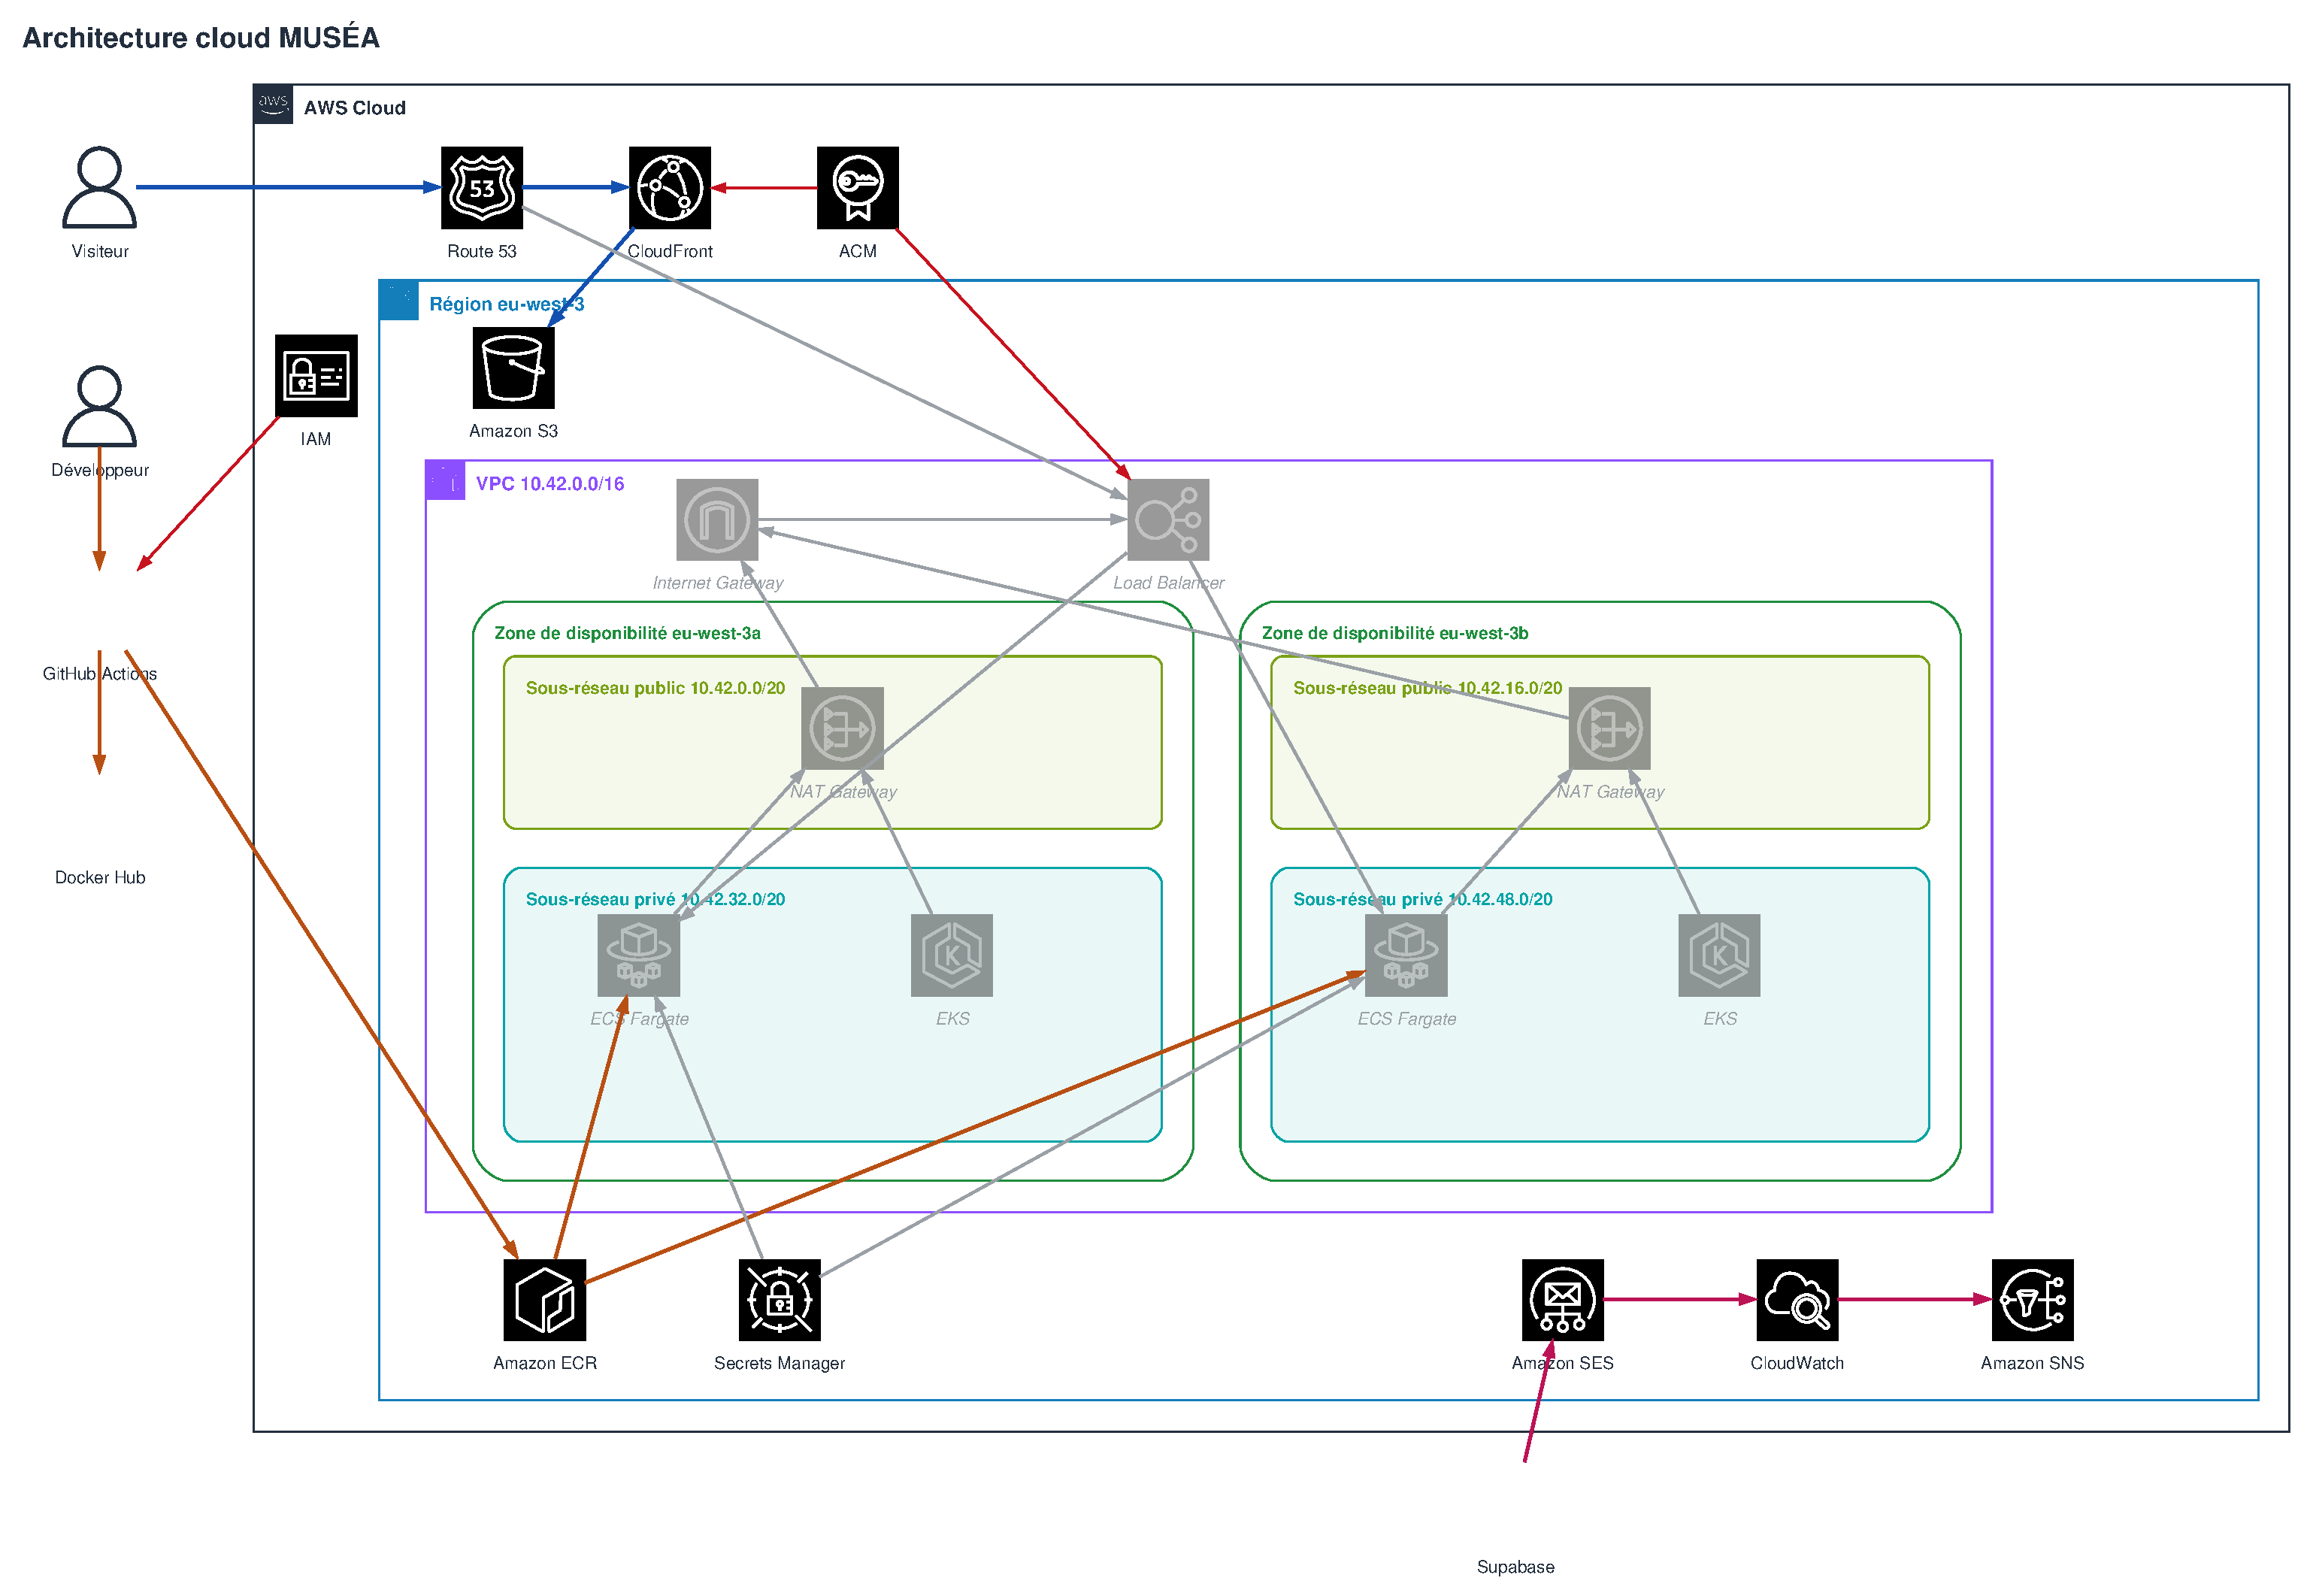
\includegraphics[width=\textwidth]{figures/architecture-cloud-musea.pdf}
\caption{Architecture de l'infrastructure d'hébergement en nuage}
\label{fig:cloud}
\source{Élaboré par nos soins d'après la description Terraform du projet.}
\end{figure}

\subsubsection{La chaîne d'intégration et de déploiement continus}

La chaîne mise en place comporte deux enchaînements.

Le premier, déclenché à chaque dépôt de modification, compile l'application et
exécute une série de contrôles sur le résultat produit : présence des fichiers
attendus, validité des modèles tridimensionnels, présence de l'adresse du
service de données dans le paquet compilé. Ce dernier contrôle mérite un mot :
sans cette adresse, le site s'affiche parfaitement et ne charge aucune donnée, la panne la plus déroutante qui soit.

Le second, déclenché sur la branche principale, publie l'application, purge le
cache de diffusion, puis, point essentiel, \textbf{vérifie le site en ligne}.
On ne contrôle pas ce que l'on croit avoir déployé, on contrôle ce que le
visiteur reçoit.

L'authentification auprès du fournisseur de nuage ne repose sur aucune clé
permanente : un jeton de courte durée est présenté à chaque exécution, et le
rôle correspondant est restreint au dépôt de code concerné, à ce seul espace de
stockage et à cette seule distribution.

La figure~\ref{fig:devops-actuel} met ces deux enchaînements en regard. La
bande supérieure est celle qui se déclenche à chaque dépôt de modification :
elle s'arrête net, sans rien publier, dès qu'un contrôle échoue. La bande
inférieure n'est atteinte que si tous les contrôles passent, et seulement
depuis la branche principale : le jeton de courte durée est alors présenté, la
publication a lieu, le cache est purgé, puis le site est vérifié \emph{en
ligne}. C'est cette dernière flèche qui distingue la chaîne d'une simple
automatisation de copie : elle interroge ce que le visiteur reçoit
effectivement, et non ce que la chaîne croit avoir déposé.

\begin{figure}[htbp]
\centering
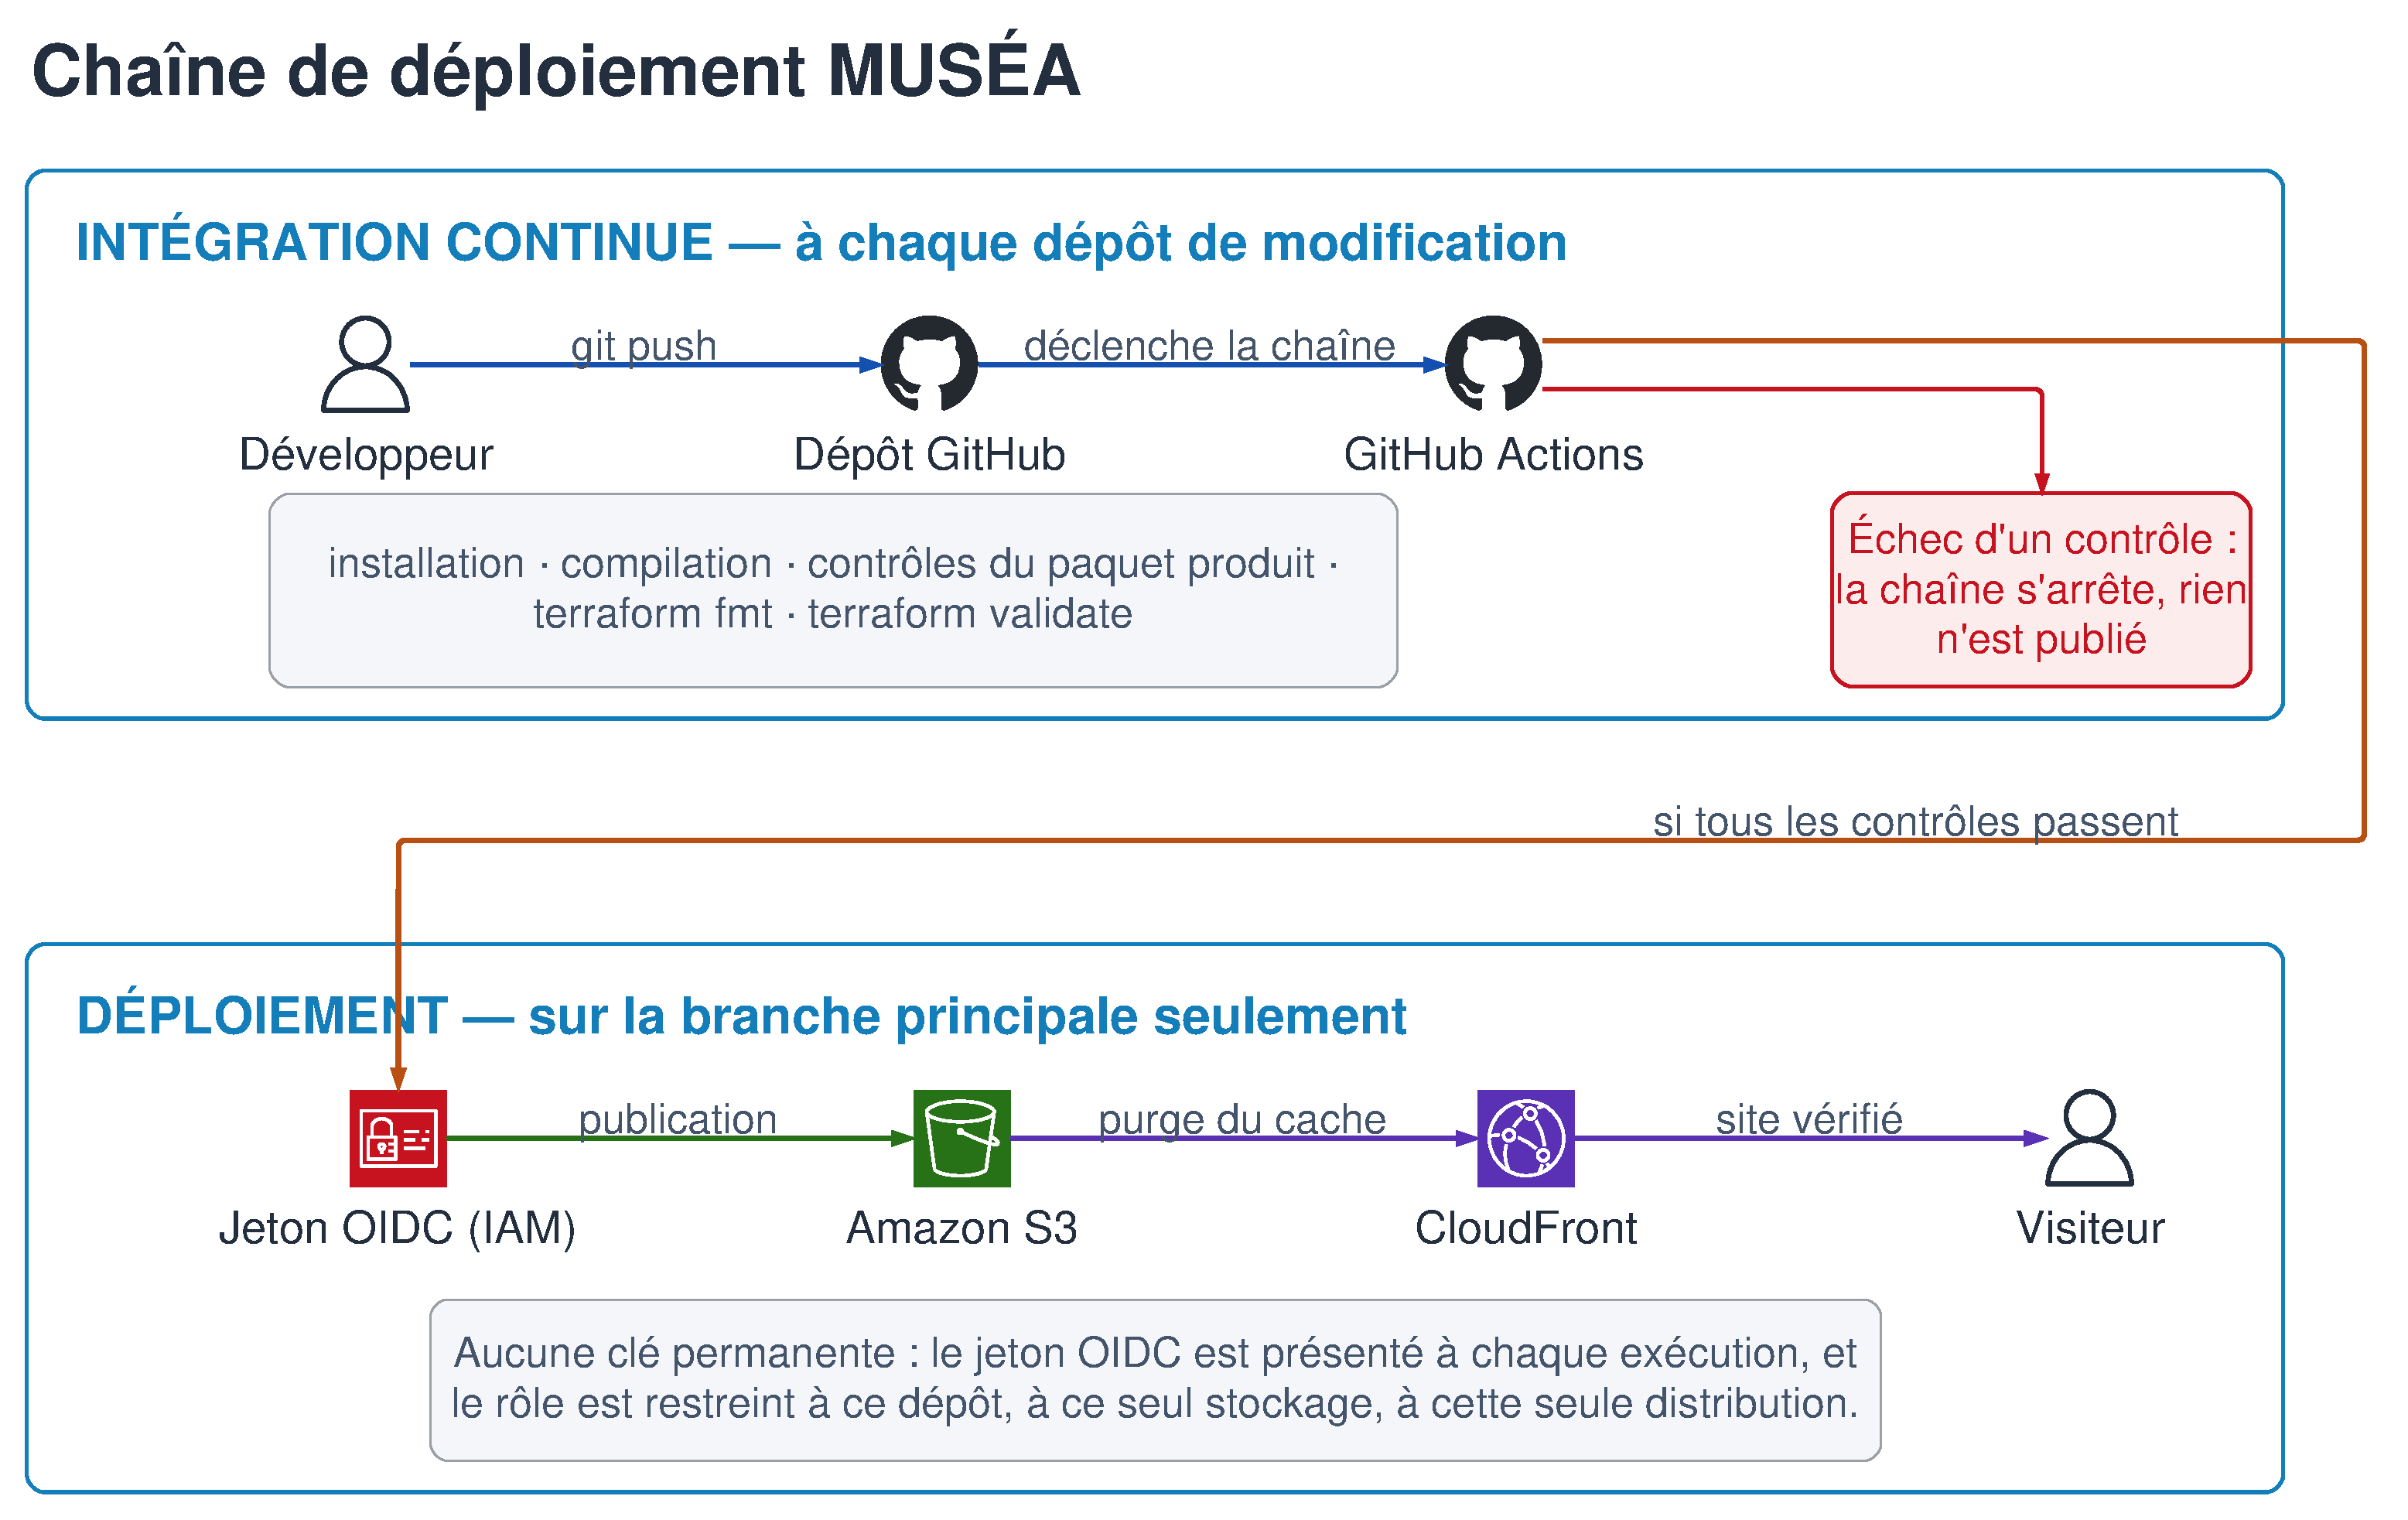
\includegraphics[width=\textwidth]{figures/deploiement-musea.pdf}
\caption{Chaîne d'intégration et de déploiement continus en service}
\label{fig:devops-actuel}
\source{Élaboré par nos soins d'après les fichiers de description des chaînes du projet.}
\end{figure}

% =============================================================================
\subsubsection{Ressources mobilisées et coût du projet}

\paragraph{Ressources matérielles.}

Le tableau~\ref{tab:materiel} recense le matériel physique mobilisé pour la
réalisation du projet.

\begin{table}[htbp]
\centering
\caption{Ressources matérielles mobilisées}
\label{tab:materiel}
\small
\begin{tabularx}{\textwidth}{|L{3.2cm}|X|C{1.3cm}|R{2.0cm}|R{2.0cm}|}
\hline
\rowcolor{keycetete}
\thead{Matériel} & \thead{Caractéristiques} & \thead{Qté} & \thead{P.U. (FCFA)} & \thead{Total (FCFA)} \\ \hline
Ordinateur portable & Processeur 8 cœurs, 32 Go de mémoire vive, 1 To de disque à semi-conducteurs & 1 & 450 000 & 450 000 \\ \hline
Écran secondaire & 24 pouces, 1920 $\times$ 1080 & 1 & 100 000 & 100 000 \\ \hline
Téléphone à capteur LiDAR & iPhone 15 Pro, acquisition tridimensionnelle et essais de réalité augmentée & 1 & 400 000 & 400 000 \\ \hline
Disque externe & 1 To, à semi-conducteurs, sauvegarde des prises de vue et des maillages & 1 & 55 000 & 55 000 \\ \hline
Onduleur & 650 VA, protection contre les coupures de courant & 1 & 48 000 & 48 000 \\ \hline
Éclairage d'appoint & 2 panneaux à diodes, prises de vue des œuvres & 1 & 45 000 & 45 000 \\ \hline
Trépied et tête panoramique & Prises de vue à 360 degrés & 1 & 35 000 & 35 000 \\ \hline
\rowcolor{keycetotal}
\multicolumn{4}{|l|}{\textbf{Coût total des ressources matérielles}} & \textbf{1 133 000} \\ \hline
\end{tabularx}
\source{Relevé des prix pratiqués à Bafoussam et à Douala, juin 2026.}
\end{table}

Le tableau~\ref{tab:materiel} appelle une lecture : l'ensemble formé par le
téléphone à capteur LiDAR et les accessoires de prise de vue (480 000 FCFA)
dépasse le poste de développement lui-même (450 000 FCFA). La contrainte
matérielle d'un tel projet tient donc à l'acquisition des images et des
volumes, non à la programmation.

\paragraph{Ressources logicielles et services.}

Le tableau~\ref{tab:logiciel} recense les logiciels et services utilisés. Il
convient de souligner que la quasi-totalité de la chaîne technique repose sur
des logiciels libres ou sur des paliers gratuits, ce qui constitue en soi un
résultat : le coût d'entrée d'un tel dispositif n'est pas logiciel, il est
matériel et humain.

\begin{table}[htbp]
\centering
\caption{Ressources logicielles et services mobilisés}
\label{tab:logiciel}
\small
\begin{tabularx}{\textwidth}{|L{4.4cm}|X|R{2.4cm}|}
\hline
\rowcolor{keycetete}
\thead{Logiciel ou service} & \thead{Rôle} & \thead{Coût (FCFA)} \\ \hline
Windows 11 Professionnel & Système d'exploitation du poste de développement & 90 350 \\ \hline
Connexion Internet & Forfait données, deux mois & 60 000 \\ \hline
Nom de domaine \texttt{.store} & Adresse publique de la plateforme, un an & 9 000 \\ \hline
Hébergement et diffusion AWS & Stockage, réseau de diffusion, noms de domaine et certificats, deux mois & 1 460 \\ \hline
Calcul graphique ponctuel & Instance à processeur graphique pour la photogrammétrie, 6 heures & 1 900 \\ \hline
Supabase & Base de données, authentification et fonctions serveur, palier gratuit & 0 \\ \hline
Groq & Génération de texte, palier gratuit & 0 \\ \hline
ElevenLabs & Synthèse vocale, palier de découverte & 0 \\ \hline
Visual Studio Code, Git, Docker, Terraform & Développement et industrialisation, logiciels libres & 0 \\ \hline
Meshroom, Blender & Photogrammétrie et préparation des maillages, logiciels libres & 0 \\ \hline
\rowcolor{keycetotal}
\multicolumn{2}{|l|}{\textbf{Coût total des ressources logicielles et services}} & \textbf{162 710} \\ \hline
\end{tabularx}
\source{Factures et relevés de consommation, juin--août 2026.}
\end{table}

Le tableau~\ref{tab:logiciel} montre que 92 \% de ce poste tient au système
d'exploitation et à la connexion Internet, c'est-à-dire à des dépenses qui
existeraient de toute façon. La chaîne technique proprement dite — base de
données, génération de texte, synthèse vocale, développement,
industrialisation — n'a rien coûté.

\paragraph{Coût de l'infrastructure en nuage.}

Le coût de l'infrastructure ne se devine pas, il se relève. Conformément aux
principes exposés au chapitre~1, la dépense a été suivie au moyen de l'outil
d'analyse des coûts du fournisseur. Le tableau~\ref{tab:finops} détaille la
dépense par service.

\begin{table}[htbp]
\centering
\caption{Détail du coût de l'infrastructure en nuage (relevé FinOps)}
\label{tab:finops}
\small
\begin{tabularx}{\textwidth}{|L{3.8cm}|X|R{2.2cm}|R{2.2cm}|}
\hline
\rowcolor{keycetete}
\thead{Service} & \thead{Usage} & \thead{Coût mensuel (FCFA)} & \thead{Sur 2 mois (FCFA)} \\ \hline
Route 53 & Zone hébergée du domaine et enregistrements joker & 310 & 620 \\ \hline
Amazon S3 & Stockage du site, des modèles 3D et des médias & 90 & 180 \\ \hline
CloudFront & Réseau de diffusion et certificat de sécurité & 330 & 660 \\ \hline
Certificate Manager & Certificats de sécurité, service gratuit & 0 & 0 \\ \hline
\rowcolor{keycetotal}
\multicolumn{2}{|l|}{\textbf{Total hébergement récurrent}} & \textbf{730} & \textbf{1 460} \\ \hline
EC2 (processeur graphique) & Reconstruction photogrammétrique, 6 heures, instance arrêtée hors usage & — & 1 900 \\ \hline
\rowcolor{keycetotal}
\multicolumn{3}{|l|}{\textbf{Total infrastructure sur la période du stage}} & \textbf{3 360} \\ \hline
\end{tabularx}
\source{AWS Cost Explorer, période du 20 juin au 20 août 2026 (voir
figure~\ref{fig:finops}).}
\end{table}

\begin{figure}[htbp]
\centering
\acapturer{5.2cm}{Insérer la capture d'écran d'AWS Cost Explorer montrant la
dépense mensuelle ventilée par service sur la période du stage. Veiller à ce que
les montants et les noms de services soient lisibles, et à masquer tout
identifiant de compte.}
\caption{Relevé de la dépense mensuelle d'infrastructure par service}
\label{fig:finops}
\source{Console AWS Cost Explorer, août 2026.}
\end{figure}

Ce relevé appelle un commentaire qui dépasse la simple comptabilité. Le coût
récurrent de l'hébergement s'établit à environ \textbf{730 FCFA par mois}, soit
moins de 9 000 FCFA par an. Ce montant, dérisoire au regard du budget d'une
institution, tient à un choix d'architecture : l'application étant un site
statique servi par un réseau de diffusion, elle ne mobilise aucun serveur en
fonctionnement permanent. Le seul poste réellement coûteux, le calcul graphique
nécessaire à la photogrammétrie, est ponctuel et l'instance correspondante
s'arrête automatiquement lorsqu'elle n'est pas sollicitée. C'est là l'apport
concret de la démarche FinOps : non pas économiser après coup, mais concevoir de
telle sorte que la dépense reste proportionnée à l'usage réel.

\paragraph{Coût total du projet.}

\begin{table}[htbp]
\centering
\caption{Coût total du projet}
\label{tab:couttotal}
\small
\begin{tabularx}{\textwidth}{|X|R{3.4cm}|}
\hline
\rowcolor{keycetete}
\thead{Libellé} & \thead{Montant (FCFA)} \\ \hline
Ressources matérielles & 1 133 000 \\ \hline
Ressources logicielles et services & 162 710 \\ \hline
Sous-total & 1 295 710 \\ \hline
Marge d'erreur (3 \%) & 38 871 \\ \hline
\rowcolor{keycetotal}
\textbf{Coût total du projet} & \textbf{1 334 581} \\ \hline
\end{tabularx}
\source{Élaboré par nos soins à partir des tableaux~\ref{tab:materiel}
et~\ref{tab:logiciel}.}
\end{table}

Le tableau~\ref{tab:couttotal} montre que 85 \% du coût total est constitué de
matériel réutilisable, acquis une fois pour toutes. La reconduction du
dispositif dans une autre institution ne suppose donc pas de reproduire cette
dépense : elle n'appelle que le coût récurrent d'hébergement relevé au
tableau~\ref{tab:finops}.

\subsection{Les résultats obtenus}
\label{sec:resultats}

Cette section décrit chacune des fonctionnalités effectivement livrées et, pour
chacune, la finalité qu'elle poursuit.

\subsubsection{F1 : La gestion des collections}

\textbf{Ce que fait la fonctionnalité.} Le back-office permet d'enregistrer les
musées, puis les salles qui les composent, puis les œuvres qu'abritent ces
salles. Chaque œuvre porte un nom, un nom commun, une description, une histoire,
des médias, une grille tarifaire, un indice de rareté et, le cas échéant, ses
modèles tridimensionnels.

\textbf{Pourquoi elle existe.} Elle constitue le socle de tout le reste : sans
inventaire structuré, ni la visite immersive, ni l'assistant, ni le
rapprochement documentaire ne disposent de matière. Elle répond directement à
l'absence de système de gestion relevée lors de l'étude de l'existant.

\subsubsection{F2 : Le site public de l'institution}

\textbf{Ce que fait la fonctionnalité.} Chaque institution dispose d'un site
public présentant son identité, ses musées, son catalogue, ses événements et sa
boutique.

\textbf{Pourquoi elle existe.} Pour que l'institution reste maîtresse de son
image. L'ensemble des éléments visibles, marque, couleurs, images d'accueil,
textes des pages de connexion, blocs de la page d'accueil, est modifiable
depuis le back-office. Aucun texte n'est figé dans le code : une institution qui
change de charte graphique n'a pas besoin d'un développeur.

\subsubsection{F3 : La visite immersive à 360 degrés}

\textbf{Ce que fait la fonctionnalité.} Le visiteur entre dans une salle,
pivote librement, zoome, passe à la salle suivante par un point de passage, et
touche un objet pour en ouvrir la fiche. Une mini-carte et une barre de
progression lui indiquent où il se trouve dans le parcours.

\textbf{Pourquoi elle existe.} Elle répond à l'attente la plus fréquemment
exprimée par les visiteurs interrogés, se déplacer dans les salles comme si
l'on y était, et à la première limite relevée dans la problématique : la visite
passive sans sensation d'espace.

\textbf{Point de conception notable.} Un mode de démonstration dessine une salle
stylisée au vol, avec plafond, cimaise, alcôves éclairées et sol, dans une
teinte différente par salle. Le parcours est donc démontrable \emph{avant} les
prises de vue réelles, ce qui, sur un terrain dépourvu de matière numérique
préexistante, a conditionné la possibilité même de présenter le dispositif.

\begin{figure}[htbp]
\centering
\acapturer{5.2cm}{Insérer la capture d'écran du parcours immersif côté visiteur :
panorama à 360 degrés, points d'intérêt cliquables, mini-carte, barre de
progression et fiche flottante d'une œuvre.}
\caption{Site public : le parcours de visite immersive}
\label{fig:cap-tour}
\source{Capture d'écran de la plateforme MUSÉA, août 2026.}
\end{figure}

\subsubsection{F4 et F5 : La présentation en trois dimensions et la réalité augmentée}

\textbf{Ce que font les fonctionnalités.} Depuis la fiche d'une œuvre, le
visiteur fait pivoter le modèle tridimensionnel, l'examine sous tous ses angles,
puis, s'il utilise un téléphone compatible, le pose dans son propre
environnement, à ses dimensions véritables.

\textbf{Pourquoi elles existent.} Pour répondre à la deuxième attente des
visiteurs et pour donner corps à ce que nous avons appelé le « retour au pays » :
faire apparaître, dans le salon d'un membre de la diaspora, un objet conservé à
Bangoulap, à sa taille réelle. Une photographie ne produit jamais cet effet.

\textbf{Couverture des appareils.} La fonction est opérationnelle sur les trois
familles d'appareils visées : Android équipé d'ARCore, sans condition ; iPhone et
iPad, dès qu'un modèle au format USDZ est chargé sur l'œuvre ; Android dépourvu
de l'interface WebXR, à condition que les modèles soient des fichiers statiques
et non des adresses temporaires. Sur ordinateur, où la réalité augmentée n'a pas
de sens, un code QR renvoie le visiteur vers son téléphone.

\subsubsection{F6 : Les codes QR de passage à l'appareil mobile}

\textbf{Ce que fait la fonctionnalité.} Un code QR affiché à l'écran renvoie
vers une page autonome dédiée à la réalité augmentée pour l'œuvre concernée.

\textbf{Pourquoi elle existe.} Parce que la réalité augmentée exige un téléphone
tandis qu'une présentation se tient devant un ordinateur. Sans ce pont, la
fonctionnalité la plus démonstrative du projet resterait invisible au public
auquel on la présente.

\subsubsection{F7 : Le relief 2.5D}

\textbf{Ce que fait la fonctionnalité.} Une photographie plate révèle du volume
lorsque l'utilisateur bouge : les sommets d'un maillage subdivisé sont déplacés
selon une carte de profondeur estimée.

\textbf{Pourquoi elle existe.} Toutes les œuvres ne seront jamais numérisées en
trois dimensions : l'opération est longue et suppose de manipuler la pièce. Le
relief offre un intermédiaire entre la photographie plate et le modèle complet.

\textbf{Limite assumée.} L'illusion tient de face et s'effondre de profil.
L'angle de parallaxe est donc borné à vingt degrés, au-delà desquels les zones
absentes de la photographie apparaissent et s'étirent. Ce bridage est la
condition du procédé, non un réglage de confort.

\subsubsection{F8 : L'assistant conversationnel à ancrage documentaire}

\textbf{Ce que fait la fonctionnalité.} Le visiteur pose une question en
français ou en anglais ; l'assistant répond à partir des documents de
l'institution, cite ses sources et propose des liens vers les fiches concernées.

\textbf{Pourquoi elle existe.} Pour répondre à la troisième limite de la
problématique, l'absence d'aide face aux questions précises, sans encourir le
risque que redoutait le personnel : qu'un dispositif automatique énonce des
contrevérités sur le patrimoine.

\textbf{Garde-fous mis en place.} Quatre mécanismes concourent à la fiabilité :
un refus poli des sujets hors périmètre, prononcé sans même solliciter le modèle
de langue ; une réponse chaleureuse aux salutations, plutôt qu'une demande de
précision déplacée ; une restriction de la recherche au musée ou à la salle où
se trouve le visiteur ; et une consigne interdisant d'énoncer un fait absent des
documents fournis, assortie de l'autorisation explicite de déclarer son
ignorance.

\subsubsection{F9 et F10 : Le guide vocal et le journal des questions}

\textbf{Ce que font les fonctionnalités.} La première permet d'écouter le récit
d'une œuvre ou d'une salle, avec une voix choisie par l'institution et pouvant
varier d'un musée, voire d'une salle, à l'autre. La seconde consigne de manière
anonyme les questions auxquelles l'assistant n'a pu répondre, les classe en huit
thèmes (matière, datation, origine, usage, auteur, dimensions, valeur,
conservation) et les présente au personnel sous forme de conseils.

\textbf{Pourquoi elles existent.} Le guide vocal répond au fait que la médiation
muséale est d'abord orale et que l'écoute libère le regard : on ne peut pas lire
une notice et observer une œuvre en même temps. Le journal, lui, retourne le
dispositif au profit de l'institution : au lieu de constater un échec, il
indique quoi documenter. Un conseil tel que « précisez la matière et la
technique de fabrication » est directement actionnable, là où un simple décompte
ne le serait pas.

\subsubsection{F11 et F12 : La mémoire réunifiée et le cabinet de comparaison}

\textbf{Ce que font les fonctionnalités.} À partir de la notice d'une œuvre, le
système interroge en parallèle cinq collections ouvertes, ordonne les résultats
par proximité de sens, fait justifier les rapprochements les plus probables,
puis les soumet au conservateur qui valide, écarte ou corrige la justification.
Les correspondances validées apparaissent alors sur la fiche publique de
l'œuvre, avec le nom du musée détenteur et le numéro d'inventaire.

\textbf{Pourquoi elles existent.} Pour répondre à la deuxième limite de la
problématique, des objets isolés et une histoire incomplète, et au thème
inattendu apparu lors des entretiens.

\textbf{Résultat marquant.} Une mesure comparative conduite sur les mêmes
collections et au même seuil de notation établit ce qui suit : une recherche
formulée directement en français ramène 16 résultats dont le meilleur atteint un
score de 57 sur 100, tandis que la même recherche reformulée dans le vocabulaire
de catalogage anglais n'en ramène que 5, mais dont le meilleur atteint 85. Ce
résultat est développé et interprété au chapitre~4.

\subsubsection{F13 : La généalogie navigable}

\textbf{Ce que fait la fonctionnalité.} Un arbre bidirectionnel présente les
ascendants à gauche, les descendants à droite et la personne consultée au
centre. Un clic recentre l'arbre sur une autre personne. Une recherche
instantanée met en évidence les cartes correspondantes. Le chemin de filiation
entre deux personnes, par l'aïeul commun le plus proche, est calculé et mis en
évidence. Une frise chronologique présente enfin la succession des règnes.

\textbf{Pourquoi elle existe.} Pour donner corps au fil narratif qui structure
tout le projet : \emph{objet $\rightarrow$ chef qui l'a possédé $\rightarrow$
chefferie $\rightarrow$ lignée $\rightarrow$ autres objets de la lignée}. Un
objet qui ne mène nulle part est un échec de conception.

\subsubsection{F14 et F15 : La billetterie et la boutique}

\textbf{Ce que font les fonctionnalités.} Le visiteur achète un billet ou un
produit d'artisanat ; le billet est délivré sous forme de code QR ; le personnel
le contrôle à l'entrée au moyen de la caméra d'un téléphone.

\textbf{Pourquoi elles existent.} Pour ouvrir un canal de recette qui n'existait
pas et pour remplacer le registre papier par un contrôle vérifiable. La boutique
répond en outre à une préoccupation exprimée par la Fondation : donner un
débouché à la production des ateliers indépendamment des visites physiques.

\subsubsection{F16 : Les adhésions et les campagnes d'information}

\textbf{Ce que fait la fonctionnalité.} Un visiteur qui crée un compte sur le
site d'une institution en devient l'adhérent. L'institution dispose alors d'un
fichier exportable et peut lui adresser des campagnes d'information, dont la
rédaction peut être assistée.

\textbf{Pourquoi elle existe.} Pour transformer une visite ponctuelle en
relation durable, ce que l'absence de fichier de visiteurs interdisait
totalement.

\textbf{Garanties apportées.} Les destinataires sont calculés par la base de
données et restreints aux adhérents ayant consenti à être contactés ; chaque
message comporte un lien de désinscription ; le contenu saisi par
l'administrateur est intégralement échappé, de sorte qu'aucun code ne puisse y
être injecté ; et la rédaction assistée se voit interdire d'inventer une date,
un horaire, un tarif ou un nom d'œuvre qui ne lui aurait pas été fourni.

\subsubsection{F17 : Le cloisonnement multi-organisations}

\textbf{Ce que fait la fonctionnalité.} Chaque institution vit sur son propre
sous-domaine et ne voit que ses propres données. Trois cercles d'identité
coexistent sans jamais se confondre : le super-administrateur de la plateforme,
le personnel d'une institution, et le visiteur, lequel possède un compte global
et adhère à une ou plusieurs institutions.

\textbf{Pourquoi elle existe.} Pour répondre au quatrième objectif : permettre
l'accueil de nouvelles institutions sans reconstruction. C'est la condition de
la diffusion du dispositif au-delà de la Fondation.

\textbf{Point de conception notable.} Le cloisonnement est appliqué par la base
de données au moyen de règles de sécurité au niveau de la ligne, et non par le
code de l'application. La différence est décisive : même un composant détourné
ou défectueux ne peut pas lire les données d'une autre institution, parce que
c'est la base qui refuse, et non le programme qui s'abstient de demander.

\subsubsection{F18 : L'assistant d'installation}

\textbf{Ce que fait la fonctionnalité.} Une institution qui vient de s'inscrire
décrit ses collections en langage courant ; un agent crée pour elle les musées,
les salles et les premières œuvres.

\textbf{Pourquoi elle existe.} Parce que la page blanche est le premier obstacle
à l'adoption. Une institution qui doit saisir cent notices avant de voir quoi
que ce soit abandonne.

\textbf{Garantie de sécurité.} L'agent écrit avec le jeton de la personne qui
l'utilise, jamais avec une clé privilégiée. Les règles de cloisonnement
s'appliquent donc exactement comme si la personne cliquait elle-même : un agent
détourné par une consigne malveillante ne peut rien écrire hors de son
institution. Les outils dont il dispose sont en outre limités à une liste
blanche, création de musée, de salle, d'œuvre et d'identité, sans aucune
suppression, et le nombre de créations est plafonné.

\subsubsection{F19 et F20 : Les statistiques de fréquentation et la carte de partage}

\textbf{Ce que font les fonctionnalités.} La première comptabilise les
consultations des fiches d'œuvres et met automatiquement en avant, sur la page
d'accueil, les pièces les plus regardées. La seconde produit une image carrée
prête à être partagée sur les messageries, comportant la photographie de
l'œuvre, son nom, sa salle, la marque de l'institution et un code QR renvoyant
vers sa fiche.

\textbf{Pourquoi elles existent.} L'une et l'autre travaillent sans que le
personnel ait à saisir, à consulter ou à décider quoi que ce soit, critère
retenu pour juger de leur utilité réelle dans une institution aux effectifs
restreints.

% =============================================================================
\subsubsection{Synthèse des mesures}

Le tableau~\ref{tab:mesures} rassemble les mesures relevées sur le système, qui
serviront de base à la vérification des hypothèses au chapitre suivant.

\begin{table}[htbp]
\centering
\caption{Synthèse des mesures relevées sur le système}
\label{tab:mesures}
\small
\begin{tabularx}{\textwidth}{|C{2.2cm}|X|C{3.0cm}|}
\hline
\rowcolor{keycetete}
\thead{Variable} & \thead{Indicateur} & \thead{Valeur relevée} \\ \hline
Variable 1 & Dimensions mesurées sur le modèle de démonstration & 45 $\times$ 52 $\times$ 45 cm \\ \hline
Variable 1 & Sommets du maillage de démonstration & 835 \\ \hline
Variable 1 & Plateformes couvertes pour la réalité augmentée & 3 sur 3 \\ \hline
Variable 1 & Angle de parallaxe admissible pour le relief & $\pm$ 20\textdegree \\ \hline
Variable 2 & Collections ouvertes effectivement interrogées & 5 \\ \hline
Variable 2 & Œuvres apparentées identifiées & 41 \\ \hline
Variable 2 & Meilleur score de correspondance obtenu & 90 / 100 \\ \hline
Variable 2 & Pays représentés sur le globe de dispersion & 137 \\ \hline
Variable 2 & Score en recherche française brute (meilleur) & 57 / 100 \\ \hline
Variable 2 & Score après reformulation en vocabulaire de catalogue & 85 / 100 \\ \hline
Variable 2 & Séparation des scores en anglais (frères / bruit) & 0,898 / 0,779 \\ \hline
Variable 2 & Séparation des scores en français (étendue) & 0,13 \\ \hline
Variable 3 & Fonctions serveur déployées & 12 \\ \hline
Variable 3 & Fragments vectorisables par appel & 18 (lots de 12 retenus) \\ \hline
Variable 3 & Durée de vectorisation de 18 fragments & 1,7 s \\ \hline
Variable 3 & Thèmes de classement des questions sans réponse & 8 \\ \hline
Variable 4 & Tables de la base de données & 38 \\ \hline
Variable 4 & Ressources d'infrastructure décrites par le code & 29 \\ \hline
Variable 4 & Ressources effectivement créées à la mise en ligne & 19 \\ \hline
Variable 4 & Coût récurrent mensuel de l'hébergement & 730 FCFA \\ \hline
\end{tabularx}
\source{Mesures effectuées sur la plateforme, juillet--août 2026.}
\end{table}

Ces vingt indicateurs se répartissent sur les quatre variables de l'étude, à
raison de quatre indicateurs pour les variables 1, 3 et 4 et de huit pour la
variable 2, la plus instrumentée. Trois d'entre eux seront particulièrement
mobilisés au chapitre suivant : la couverture des trois familles d'appareils
pour la variable 1, l'écart entre les scores obtenus en français et en anglais
pour la variable 2, et le coût récurrent mensuel pour la variable 4.

\conclchap

Ce chapitre a présenté le site de l'étude — la Fondation Jean Félicien Gacha,
son Département \emph{Think Tank} Fou'ndjem et le rôle exact que celui-ci a tenu
dans le projet —, le déroulement du stage, les données recueillies auprès du
personnel et des visiteurs, l'implémentation du dispositif et les vingt
fonctionnalités livrées.

Deux enseignements s'en dégagent. D'une part, les insuffisances relevées lors de
l'étude de l'existant, les thèmes issus des entretiens et les attentes mesurées
auprès des visiteurs convergent vers les mêmes priorités, dans le même ordre :
se déplacer dans les espaces, percevoir les objets, interroger, relier. D'autre
part, le dispositif construit à partir de ces données a effectivement été livré
et mesuré. Les mesures rassemblées en fin de chapitre constituent la matière
factuelle du diagnostic, que le chapitre~\ref{chap:diagnostic} interprète au
regard des hypothèses de l'étude.
